\expandafter\let\csname ver@amssymb.sty\endcsname\empty
\documentclass[serif]{beamer}
\expandafter\let\csname ver@amssymb.sty\endcsname\relax
\usepackage{etex}
\usepackage[bitstream-charter]{mathdesign} % Use BT Charter font
\usepackage[T1]{fontenc}                   % Use T1 encoding instead of OT1
\usepackage[utf8]{inputenc}                % Use UTF8 input encoding
\usepackage{microtype}                     % Improve typography
\usepackage{booktabs}
\usepackage{cancel}
\usepackage{algorithm}
\usepackage{algorithmicx}
\usepackage{algpseudocode}
\usepackage{hyperref}
\hypersetup{pdfstartview=Fit}
\usepackage{tikz}
\usetikzlibrary{shapes,snakes,shadows,arrows,calc}
\usepackage{multirow}
\usepackage{animate}
\usepackage{moresize}
\usepackage{colortbl}
\usepackage{xcolor}
\usepackage{amsmath}
\usepackage{etoolbox}
\usepackage{listings}
\usepackage{alltt}

\renewcommand\footnotemark{}

\lstset{
  columns=fullflexible,
  showspaces=false,
  showtabs=false,
  showstringspaces=false,
  commentstyle=\color{gray}\upshape,
}
\lstset{language=bash,frame=single,basicstyle=\ttfamily\footnotesize}
\lstdefinelanguage{XML}
{
  backgroundcolor=\color{gray!20},
  basicstyle=\ttfamily\ssmall,
  morestring=[b]",
  frame=single,
% morestring=[s]{>}{<},
  morecomment=[s]{<?}{?>},
  morecomment=[s]{<!--}{-->},
  stringstyle=\color{red},
  identifierstyle=\color{darkblue},
  keywordstyle=\color{cyan},
}

\definecolor{gray}{rgb}{0.4,0.4,0.4}
\definecolor{darkblue}{rgb}{0.0,0.0,0.6}
\definecolor{cyan}{rgb}{0.0,0.6,0.6}

\newcommand{\tikzmark}[1]{\tikz[overlay,remember picture] \node (#1) {};}
\newcommand*{\DrawArrow}[3][]{%
    % #1 = draw options
    % #2 = left point
    % #3 = right point
    \begin{tikzpicture}[overlay,remember picture]
        \draw [-latex, #1] ($(#2)+(0.3em,-1ex)$) to ($(#3)+(0,0.5ex)$);
    \end{tikzpicture}%
}

\usetheme{Copenhagen}
\usecolortheme{beaver}

\title{OpenMC Module: Basic Model Building}
\author{\emph{Computational Reactor Physics Group}}
\date{\normalsize Department of Nuclear Science and Engineering\\
                  Massachusetts Institute of Technology \\
~\\
\tiny{This work is licensed under the Creative Commons Attribution-ShareAlike 3.0 Unported License. To view a copy of this license, visit http://creativecommons.org/licenses/by-sa/3.0/.}}
% Set Logo
\logo{
\includegraphics[scale=0.2]{src/crpg.png}\hspace*{8cm}

\includegraphics[scale=0.2,trim=0cm 3.0cm 2.2cm 0cm, clip=true]{src/mitlogo.pdf}}

\usenavigationsymbolstemplate{}

%-------------------------------------------------------------------------------
\begin{document}
%-------------------------------------------------------------------------------

\frame{\titlepage}\logo{} % remove logo after title page

%-------------------------------------------------------------------------------

\begin{frame}{Problem to Solve}
  \begin{itemize}
     \item<1-> Simple pin-cell comprised of $\rm{UO}_2$, clad and water
     \vfill
     \item<1-> \textbf{Objective}: Deterimine $k_{eff}$ of pin-cell 
  \end{itemize}
  \vfill
  \vfill
  \begin{columns}
    \begin{column}{0.3\linewidth}
      \def\Scale{2.5}
      \begin{tikzpicture}
        \draw[fill=blue] (-.63339cm*\Scale,-.63339cm*\Scale) rectangle 
                         (0.63339cm*\Scale,0.63339cm*\Scale);
        \draw[fill=yellow] (0cm,0cm) circle (0.45972cm*\Scale);
        \draw[fill=green] (0cm,0cm) circle (0.40226cm*\Scale);
        \draw[fill=red] (0cm,0cm) circle (0.39433cm*\Scale);
        \draw[fill=red] (-0.6cm*\Scale,-0.8cm*\Scale) rectangle 
                        (-0.55cm*\Scale,-0.75cm*\Scale);
        \node at (-0.41cm*\Scale,-0.78cm*\Scale) {Fuel};
        \draw[fill=yellow] (-0.2cm*\Scale,-0.8cm*\Scale) rectangle 
                           (-0.15cm*\Scale,-0.75cm*\Scale);
        \node at (0.0cm*\Scale,-0.78cm*\Scale) {Clad};
        \draw[fill=blue] (0.20cm*\Scale,-0.8cm*\Scale) rectangle 
                         (0.25cm*\Scale,-0.75cm*\Scale);
        \node at (0.45cm*\Scale,-0.78cm*\Scale) {Water};
      \end{tikzpicture}
    \end{column}
    \begin{column}{0.7\linewidth}
      \footnotesize
      \begin{tabular}{l l c}
        \toprule
        Material & Isotope & Composition Fraction (a or w) \\
        \midrule
        \midrule
        Fuel & U-235 & 0.02115 (w) \\
        Fuel & U-238 & 0.86032 (w) \\
        Fuel & O-16  & 0.11852 (w) \\
        \midrule
        Clad & Zr & elemental \\
        \midrule
        Water & H-1  & 2.0 (a) \\
        Water & O-16 & 1.0 (a) \\
        \bottomrule
      \end{tabular}
      {\centering\footnotesize w = weight fraction, a = atom fraction}
    \end{column}
  \end{columns}
\end{frame}

%-------------------------------------------------------------------------------

\begin{frame}{Creating Geometry in OpenMC}
  \begin{itemize}
    \vfill
    \item<1-> OpenMC uses constructive solid geometry
    \vfill
    \item<1-> Intersections of surfaces are used to create cells
  \end{itemize}
  \vfill
  \begin{columns}[T]
    \begin{column}[T]{0.5\linewidth}
      \begin{itemize}
        \item<1-> List of surface types:
        \begin{itemize}
          \item<1-> x-, y-, z-plane
          \vfill
          \item<1-> general plane
          \vfill
          \item<1-> x-, y-, z-cylinder
          \vfill
          \item<1-> sphere
          \vfill
          \item<1-> x-, y-, z-cone
        \end{itemize}
        \vfill
        \item<1-> Each surface type takes difference arguments
      \end{itemize}
    \end{column}
    \begin{column}[T]{0.5\linewidth}
      \vfill
      \begin{center}
        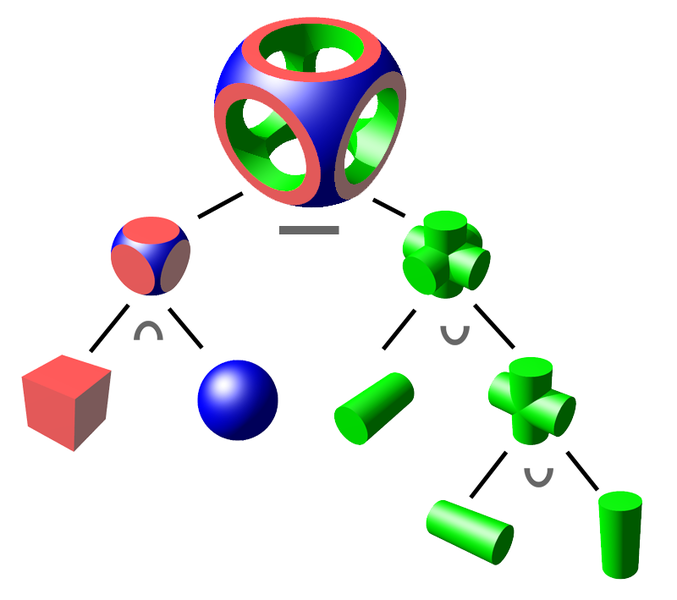
\includegraphics[scale=0.15]{src/csg-tree.png} \\
        \scriptsize
        source: Wikipedia
      \end{center}
    \end{column}
  \end{columns}
\end{frame}

%-------------------------------------------------------------------------------

\begin{frame}[fragile]{Pin-cell Surface Definitions}

  \begin{scriptsize}
    \begin{lstlisting}[language=XML]
      <surface id="1" type="z-cylinder" coeffs="0.0 0.0 0.39218" />
      <surface id="2" type="z-cylinder" coeffs="0.0 0.0 0.40005" />
      <surface id="3" type="z-cylinder" coeffs="0.0 0.0 0.45720" />
      <surface id="4" type="x-plane"    coeffs="-0.62992" boundary="reflective" />
      <surface id="5" type="x-plane"    coeffs=" 0.62992" boundary="reflective" />
      <surface id="6" type="y-plane"    coeffs="-0.62992" boundary="reflective" />
      <surface id="7" type="y-plane"    coeffs=" 0.62992" boundary="reflective" />
      <surface id="8" type="z-plane"    coeffs="-5.0"     boundary="reflective" />
      <surface id="9" type="z-plane"    coeffs=" 5.0"     boundary="reflective" /> 
    \end{lstlisting}
  \end{scriptsize}
  \vfill
  \begin{center}
    \scalebox{0.5}{
    \begin{tikzpicture}[scale=8,auto]
      \draw (0,0) circle (0.39218);
      \draw[->] (0,0) -- node[pos=0.65] {1} (0.196,0.34);
      \draw (0,0) circle (0.40005);
      \draw[->] (0,0) -- node[pos=0.65] {2} (-0.346,0.2);
      \draw (0,0) circle (0.4572);
      \draw[->] (0,0) -- node[pos=0.65] {3} (0.3232,-0.3232);
      \draw (-0.63,-0.63) rectangle (0.63,0.63);
      \draw[->] (0,0) -- node[pos=0.85] {4} (0.63,0.0);
      \draw[->] (0,0) -- node[pos=0.85] {5} (-0.63,0.0);
      \draw[->] (0,0) -- node[pos=0.85] {6} (0.0,-0.63);
      \draw[->] (0,0) -- node[pos=0.85] {7} (0.0,0.63); 
    \end{tikzpicture}}
  \end{center}

\end{frame}

%-------------------------------------------------------------------------------

\begin{frame}[fragile]{Pin-cell Cell Definitions}

  \begin{scriptsize}
    \begin{lstlisting}[language=XML]
      <cell id="1" material="1"    surfaces="-1 8 -9"          /> 
      <cell id="2" material="void" surfaces="1 -2 8 -9"        />
      <cell id="3" material="2"    surfaces="2 -3 8 -9"        />
      <cell id="4" material="3"    surfaces="3 4 -5 6 -7 8 -9" />
    \end{lstlisting}
  \end{scriptsize}
  \vfill
  \begin{columns}
    \begin{column}{0.3\linewidth}
      \begin{center}
        \scalebox{0.3}{
        \begin{tikzpicture}[scale=8,auto]
          \draw[fill=blue] (-0.63,-0.63) rectangle (0.63,0.63);
          \draw[fill=yellow] (0,0) circle (0.4572);
          \draw[fill=green] (0,0) circle (0.40005);
          \draw[fill=red] (0,0) circle (0.39218);
        \end{tikzpicture}}
      \end{center}
    \end{column}
    \begin{column}{0.4\linewidth}\footnotesize
	  \begin{itemize}
        \item<1-> {\color{red} Fuel} --- Material 1
        \begin{itemize}\scriptsize
           \item<1-> Inside Surface 1 (-1)
           \item<1-> Above -z plane (8)
           \item<1-> Below +z plane (-9)
        \end{itemize}
        ~\\
        ~\\
        \item<1-> {\color{green} Gap} --- No Material (\emph{void})
        \begin{itemize}\scriptsize
           \item<1-> Outside Surface 1 (1)
           \item<1-> Inside Surface 2 (-2) 
           \item<1-> Above -z plane (8)
           \item<1-> Below +z plane (-9)
        \end{itemize}
      \end{itemize}
    \end{column}
    \begin{column}{0.4\linewidth}\footnotesize
      \begin{itemize}
        \item<1-> {\color{yellow!80!black} Clad} --- Material 2
        \begin{itemize}\scriptsize
           \item<1-> Outside Surface 2 (2)
           \item<1-> Inside Surface 3 (-3) 
           \item<1-> Above -z plane (8)
           \item<1-> Below +z plane (-9)
        \end{itemize}\vfill
        \item<1-> {\color{blue} Coolant} --- Material 3
        \begin{itemize}\scriptsize
           \item<1-> Outside Surface 3 (3)
           \item<1-> Right -x plane (4)
           \item<1-> Left +x plane (-5)
           \item<1-> Above -y plane (6)
           \item<1-> Below +y plane (-7)
           \item<1-> Above Bottom (8)
           \item<1-> Below Top (-9)
        \end{itemize}
      \end{itemize}
    \end{column}
  \end{columns}

\end{frame}

%-------------------------------------------------------------------------------

\begin{frame}[fragile]{Pin-cell \texttt{geometry.xml} File}
  \vfill
  \begin{scriptsize}
    \begin{lstlisting}[language=XML]
      <?xml version="1.0" encoding="UTF-8"?>
      <geometry>

        <!-- Surfaces -->
        <surface id="1" type="z-cylinder" coeffs="0.0 0.0 0.39218" /> <!-- fuel radius -->
        <surface id="2" type="z-cylinder" coeffs="0.0 0.0 0.40005" /> <!-- clad iradius -->
        <surface id="3" type="z-cylinder" coeffs="0.0 0.0 0.45720" /> <!-- clad oradius -->
        <surface id="4" type="x-plane"    coeffs="-0.62992" boundary="reflective" />
        <surface id="5" type="x-plane"    coeffs=" 0.62992" boundary="reflective" />
        <surface id="6" type="y-plane"    coeffs="-0.62992" boundary="reflective" />
        <surface id="7" type="y-plane"    coeffs=" 0.62992" boundary="reflective" />
        <surface id="8" type="z-plane"    coeffs="-5.0"     boundary="reflective" />
        <surface id="9" type="z-plane"    coeffs=" 5.0"     boundary="reflective" />

        <!-- Cells -->
        <cell id="1" material="1"    surfaces="-1 8 -9"          />  <!-- fuel -->
        <cell id="2" material="void" surfaces="1 -2 8 -9"        />  <!-- gas gap -->
        <cell id="3" material="2"    surfaces="2 -3 8 -9"        />  <!-- clad -->
        <cell id="4" material="3"    surfaces="3 4 -5 6 -7 8 -9" />  <!-- coolant -->

      </geometry>
    \end{lstlisting}
  \end{scriptsize}
  \vfill
\end{frame}

%-------------------------------------------------------------------------------

\begin{frame}{Creating Materials in OpenMC}

  \begin{itemize}
    \item<1-> Total density of material can be specified in units of 
              \texttt{g/cc} or \texttt{atom/b-cm}\vfill
    \item<1-> Either isotopes or natural elements (OpenMC automatically expands them)
              are specified
    \item<1-> Each isotope/element has a \texttt{\color{darkblue}name} and \texttt{\color{darkblue}xs} attribute 
              which links it to an ACE file via the \texttt{cross\_sections.xml} file
      \begin{itemize}
        \item<1-> \texttt{\color{darkblue}name} is an isotope's or element's name (e.g.,H-1 or Zr)
        \item<1-> \texttt{\color{darkblue}xs} is the ACE file cross section extension (for temperature)
      \end{itemize}
    \vfill
    \item<1-> Each isotope/element is given a weight fraction or atom fraction
              (OpenMC automatically renormalizes to a sum of one) \vfill
    \item<1-> Finally thermal scattering libraries are available with \texttt{\color{darkblue}sab} attribute
    \vfill
  \end{itemize}

\end{frame}

%-------------------------------------------------------------------------------

\begin{frame}[fragile]{Pin-cell \texttt{materials.xml} File}
  \vfill
  \begin{scriptsize}
    \begin{lstlisting}[language=XML]
      <?xml version="1.0" encoding="UTF-8"?>
      <materials>

        <!-- UO2 -->
        <material id="1">
          <density value="10.3" units="g/cc" />
          <nuclide name="U-235" xs="70c" wo="0.02115" />
          <nuclide name="U-238" xs="70c" wo="0.86032" />
          <nuclide name="O-16"  xs="70c" wo="0.11852" />
        </material>

        <!-- Zirconium -->
          <material id="2">
          <density value="6.55" units="g/cc" />
          <element name="Zr" xs="70c" ao="1" />
        </material>

        <!-- Water -->
        <material id="3">
          <density value="0.701" units="g/cc" />
          <nuclide name="H-1"  xs="70c" ao="2.0" />
          <nuclide name="O-16" xs="70c" ao="1.0" />
          <sab     name="lwtr" xs="70t" />
        </material>

      </materials>
    \end{lstlisting}
  \end{scriptsize}
  \vfill
\end{frame}

%-------------------------------------------------------------------------------

\begin{frame}{Basic OpenMC Settings for Eigenvalue Calculation}

  \begin{itemize}

    \item<1-> \texttt{\color{darkblue}cross sections} path 
              to \texttt{cross\_sections.xml} file relative to execution directory\vfill
    \item<1-> \texttt{\color{darkblue}batches}: total number of batches to run\vfill
    \item<1-> \texttt{\color{darkblue}inactive}: number of batches to discard\vfill
    \item<1-> \texttt{\color{darkblue}particles}: number of neutron histories
              per batch to simulate\vfill
    \item<1-> Initial source must be specified (e.g., from file, box/point, angle, energy)\vfill
    \begin{center}
      \alert{More options discussed in later modules and in User's Guide}
    \end{center}

  \end{itemize}

\end{frame}

%-------------------------------------------------------------------------------

\begin{frame}[fragile]{Pin-cell \texttt{settings.xml} File}

  \begin{itemize}
    \item 120 total batches, discard 20 with 1000 neutron histories per batch
    \item Starting source guess is a uniform across geometry
  \end{itemize}
  \vfill
  \begin{scriptsize}
    \begin{lstlisting}[language=XML,gobble=4]
      <?xml version="1.0" encoding="UTF-8"?>
      <settings>

        <!-- Parameters for criticality calculation -->
        <eigenvalue batches="120" inactive="20" particles="1000" />

        <!-- Starting source (default energy is Watt, default angle is isotropic) -->
        <source>
          <space type="box">
            <parameters> -0.62992 -0.62992 -5.0 0.62992 0.62992 5.0 </parameters>
          </space>
        </source>

      </settings>
    \end{lstlisting}
  \end{scriptsize}
  \vfill
\end{frame}

%-------------------------------------------------------------------------------

\begin{frame}[fragile]{Nuclide data \texttt{cross\_sections.xml} File}
  \begin{columns}
  \begin{column}{0.5\linewidth}
  \begin{itemize}
    \footnotesize
    \item {\color{darkblue}directory}: root director of ace files
    \item {\color{darkblue}alias}: \texttt{materials.xml} file links here
    \item {\color{darkblue}awr}: atomic weight ratio
    \item {\color{darkblue}location}: line number where isotope begins
  \end{itemize}
  \end{column}
  \begin{column}{0.5\linewidth}
    \footnotesize
    \begin{itemize}
      \item {\color{darkblue}name}: isotope zaid and extension
      \item {\color{darkblue}path}: relative path of ACE file from root
      \item {\color{darkblue}temperature}: isotope temp. in MeV
      \item {\color{darkblue}zaid}: isotope ZAID ID
    \end{itemize}
  \end{column}
  \end{columns}
  \vfill
  \begin{scriptsize}
    \begin{lstlisting}[language=XML,basicstyle=\ttfamily\tiny,breaklines=true]
<?xml version="1.0" ?>
<cross_sections>
  <directory>/opt/mcnp/data</directory>
  <filetype>ascii</filetype>
  <ace_table alias="H-1.70c" awr="0.999167" location="1" name="1001.70c" path="endf70a" temperature="2.5301e-08" zaid="1001"/>
  <ace_table alias="H-1.72c" awr="0.999167" location="4115" name="1001.72c" path="endf70a" temperature="7.7556e-08" zaid="1001"/>
  <ace_table alias="H-2.70c" awr="1.9968" location="10286" name="1002.70c" path="endf70a" temperature="2.5301e-08" zaid="1002"/>
  <ace_table alias="H-3.70c" awr="2.989596" location="23704" name="1003.70c" path="endf70a" temperature="2.5301e-08" zaid="1003"/>
  <ace_table awr="0.999167" location="2637033" name="lwtr.10t" path="endf70sab" zaid="0"/>
</cross_sections>
    \end{lstlisting}
  \end{scriptsize}
  \vfill
\end{frame}

%-------------------------------------------------------------------------------

\begin{frame}{Let's Run OpenMC!}

  \begin{enumerate}
    \item Make sure OpenMC is compiled
    \item Make sure you have the XML input files created
    \item Navigate to the directory containing input files
    \item Execute OpenMC!
  \end{enumerate}
  \vfill
  \begin{center}
    \alert{\{path\_to\_openmc\_root\}/src/openmc}
  \end{center}

\end{frame}

%-------------------------------------------------------------------------------

\begin{frame}[fragile]{Standard Output --- Header Information}
  \begin{columns}
  \begin{column}{0.65\linewidth}
    \begingroup
    \fontsize{4pt}{4.8pt}\selectfont
    \begin{semiverbatim}
       .d88888b.                             888b     d888  .d8888b.
      d88P" "Y88b                            8888b   d8888 d88P  Y88b
      888     888                            88888b.d88888 888    888
      888     888 88888b.   .d88b.  88888b.  888Y88888P888 888
      888     888 888 "88b d8P  Y8b 888 "88b 888 Y888P 888 888
      888     888 888  888 88888888 888  888 888  Y8P  888 888    888
      Y88b. .d88P 888 d88P Y8b.     888  888 888   "   888 Y88b  d88P
       "Y88888P"  88888P"   "Y8888  888  888 888       888  "Y8888P"
__________________888______________________________________________________
                  888
                  888

      Developed At:  Massachusetts Institute of Technology
      Version:       0.5.1
      Git SHA1:      4a5ad36f74fd2c50a7ab49a43107b610e7e6ec2c \tikzmark{end}
      Date/Time:     2013-03-23 19:55:48

 ===========================================================================
 ========================>     INITIALIZATION     <=========================
 ===========================================================================

 Reading settings XML file...
 Reading cross sections XML file...                 \tikzmark{end1}
 Reading geometry XML file...
 Reading materials XML file...
 Building neighboring cells lists for each surface...
 Loading ACE cross section table: 92235.70c
 Loading ACE cross section table: 92238.70c
 Loading ACE cross section table: 8016.70c
 Loading ACE cross section table: 40090.70c
 Loading ACE cross section table: 40091.70c
 Loading ACE cross section table: 40092.70c
 Loading ACE cross section table: 40094.70c       \tikzmark{end2}
 Loading ACE cross section table: 40096.70c
 Loading ACE cross section table: 1001.70c
 Loading ACE cross section table: lwtr.70t
 Creating unionized energy grid...
 Initializing source particles...
    \end{semiverbatim}\endgroup
  \end{column}
  \begin{column}{0.35\linewidth}
    \scriptsize
    \begin{itemize}
      \vfill
      \item Version and\tikzmark{start} execution information
      \\~
      \\~
      \item Input files\tikzmark{start1} are read and processed
      \\~
      \\~
      \item Cross sections\tikzmark{start2} are loaded into memory
      \\~
      \\~
    \end{itemize}
  \end{column}
  \end{columns}
  \DrawArrow[red, thick, out=-60, in=0]{start}{end}
  \DrawArrow[red, thick, out=-60, in=0]{start1}{end1}
  \DrawArrow[red, thick, out=-60, in=0]{start2}{end2}
\end{frame}

%-------------------------------------------------------------------------------

\begin{frame}[fragile]{Standard Output --- Header Information}
  \begin{columns}
  \begin{column}{0.65\linewidth}
    \begingroup
    \fontsize{4pt}{4.8pt}\selectfont
    \begin{semiverbatim}
 ===========================================================================
 ====================>     K EIGENVALUE SIMULATION     <====================
 ===========================================================================

  Bat./Gen.   k(batch)        Average k
  =========   ========   ====================
        1/1    1.37743\tikzmark{end}                       
        2/1    1.23928                       
           ....
       18/1    1.30948                       
       19/1    1.37513                       
       20/1    1.35739                       
       21/1    1.25861\tikzmark{end2}                       
       22/1    1.23967    1.24914 +/- 0.00947
       23/1    1.34688    1.28172 +/- 0.03303
       24/1    1.28363    1.28220 +/- 0.02336
           ....                   ...
      110/1    1.31772    1.31056 +/- 0.00453
      111/1    1.33785    1.31086 +/- 0.00449
      112/1    1.33253    1.31110 +/- 0.00444
      113/1    1.31805    1.31117 +/- 0.00439
      114/1    1.38429    1.31195 +/- 0.00442\tikzmark{end3}
      115/1    1.32248    1.31206 +/- 0.00437
      116/1    1.32758    1.31222 +/- 0.00433
      117/1    1.26614    1.31175 +/- 0.00431
      118/1    1.36733    1.31232 +/- 0.00430
      119/1    1.31629    1.31236 +/- 0.00426
      120/1    1.30628    1.31230 +/- 0.00422
 Creating state point statepoint.120.binary...\tikzmark{end4}
    \end{semiverbatim}\endgroup
    \end{column}
    \begin{column}{0.35\linewidth}
    \scriptsize
    \begin{itemize}
      \vfill
      \item Inactive Batches (tracklength k-eff reported) \tikzmark{start}
      \\~
      \\~
      \item Active Batches\tikzmark{start2} begin
      \\~
      \\~
      \item K-eff is accumulated\tikzmark{start3}
      \\~
      \\~
      \item Binary output\tikzmark{start4} file written
    \end{itemize}
  \end{column}
  \end{columns}
  \DrawArrow[red, thick, out=-160, in=0]{start}{end}
  \DrawArrow[red, thick, out=-160, in=0]{start2}{end2}
  \DrawArrow[red, thick, out=-160, in=0]{start3}{end3}
  \DrawArrow[red, thick, out=-160, in=0]{start4}{end4}
\end{frame}

%-------------------------------------------------------------------------------

\begin{frame}[fragile]{Standard Output --- Results Information}
    \begingroup
    \fontsize{6pt}{6.8pt}\selectfont
    \begin{semiverbatim}
 ===========================================================================
 ======================>     SIMULATION FINISHED     <======================
 ===========================================================================


 =======================>     TIMING STATISTICS     <=======================

 Total time for initialization     =  3.2280E+00 seconds
   Reading cross sections          =  3.0860E+00 seconds
   Unionizing energy grid          =  7.9000E-02 seconds
 Total time in simulation          =  2.5496E+01 seconds
   Time in transport only          =  2.5478E+01 seconds
   Time in inactive batches        =  4.2360E+00 seconds
   Time in active batches          =  2.1260E+01 seconds
   Time synchronizing fission bank =  6.0000E-03 seconds
     Sampling source sites         =  5.0000E-03 seconds
     SEND/RECV source sites        =  1.0000E-03 seconds
   Time accumulating tallies       =  0.0000E+00 seconds
 Total time for finalization       =  0.0000E+00 seconds
 Total time elapsed                =  2.8724E+01 seconds
 Calculation Rate                  =  4706.62 neutrons/second

 ============================>     RESULTS     <============================

 k-effective (Collision)     =  1.31513 +/-  0.00378
 k-effective (Track-length)  =  1.31230 +/-  0.00422
 k-effective (Absorption)    =  1.31639 +/-  0.00239
 Combined k-effective        =  1.31563 +/-  0.00229
 Leakage Fraction            =  0.00000 +/-  0.00000
    \end{semiverbatim}\endgroup
\end{frame}


%-------------------------------------------------------------------------------
\end{document}
%-------------------------------------------------------------------------------
